\documentclass[a4paper, titlepage, 12pt]{article}
\usepackage[margin=3.7cm]{geometry}
\usepackage[utf8]{inputenc}
\usepackage[T1]{fontenc}
% \usepackage[swedish]{babel}
\usepackage{csquotes}
\usepackage[hyphens]{url}
\usepackage{amsmath,amssymb,amsthm, amsfonts}
\usepackage[backend=biber,citestyle=ieee]{biblatex}
\usepackage{algorithm}
\usepackage{parskip}
\usepackage{float}
\usepackage{newfloat}
\usepackage{varioref, prettyref}
\usepackage{hyperref, cleveref}
\usepackage{fancyhdr}
\usepackage{multicol}
\usepackage{tocloft}
\usepackage[yyyymmdd]{datetime}
\usepackage[table]{xcolor}
\usepackage[export]{adjustbox}
\usepackage{tabularx}
\usepackage{longtable}
\usepackage{enumitem}
%\usepackage{subfig}
\usepackage{dirtree}
\usepackage{makecell}
\usepackage{hyphenat}
\usepackage{array}
\usepackage{listings}
\usepackage[font={small,it}, width=0.75\textwidth]{caption}
\usepackage[titletoc, title]{appendix}
\usepackage{seqsplit}
\usepackage{subcaption}
\usepackage{pdfpages}
\usepackage[acronym,nogroupskip,nonumberlist,nopostdot,toc]{glossaries}

\renewcommand{\dateseparator}{--}

\addbibresource{sources.bib}

%To follow Miun Template
\usepackage{mathpazo} %Set Palatino as main font
\usepackage{verbatimbox}

\usepackage{titlesec}
\usepackage{helvet}
\definecolor{thesisyellow}{HTML}{FFE500}  
\definecolor{thesisblue}{HTML}{0078BE} 
\usepackage{tikz}

\titleformat{\section}
  {\sffamily\LARGE\bfseries}{\thesection}{1em}{}
\titleformat{\subsection}
  {\sffamily\Large\bfseries}{\thesubsection}{1em}{}
\titleformat{\subsubsection}
  {\sffamily\large\bfseries}{\thesubsubsection}{1em}{}
\titleformat{\paragraph}[runin]
  {\sffamily\normalsize\bfseries}{\theparagraph}{1em}{}

% \addto\captionsenglish{
 \renewcommand{\contentsname}
   {Table of Contents}
% }

\DeclareFloatingEnvironment[placement={!ht},name=List]{mylist}

\usepackage{etoolbox}

\setcounter{tocdepth}{4}
\setcounter{secnumdepth}{4}

\newcommand{\paddedtable}[2]{\renewcommand{\arraystretch}{#1}
\begin{table}[H]\footnotesize\centering #2 \end{table}}

\newcommand{\getauthor}{Elias Berglin} %Author
\newcommand{\gettitle}{Implementing Internet of Things Protocols} %Title

\renewcommand{\headrulewidth}{0.4pt}

\begin{document}

    \begin{titlepage}
  \setlength\headheight{60pt}
  \renewcommand{\headrulewidth}{0pt}
  \thispagestyle{fancy}
  \fancyhf{}
  \rhead{
\includegraphics[width=41mm]{img/miun_logo.png}}
  \fancyfoot{}
    \vspace*{0.5cm}
    {\fontfamily{phv}\selectfont{%
    	\Large{\textbf{\gettitle}}}
      \\
      \\
      \large{} %Subtitle
    \\
    \\
    \\
    	\large{\getauthor}}
    \vspace*{13cm}

    \fontfamily{phv}
    \renewcommand{\arraystretch}{0.5}
    \begin{tabular}{l}
    \footnotesize{\textbf{MID SWEDEN UNIVERSITY}}\\
    \footnotesize{Department of Information Systems and Technology (IST)}\\
          \\

      \footnotesize{\textbf{Main field of study:} Computer Engineering }\\
      \footnotesize{\textbf{Credits:}  }\\
      \footnotesize{\textbf{Semester, year:} VT, 2022}\\
      \footnotesize{\textbf{Supervisor:} Stefan Forsström}\\
      \footnotesize{\textbf{Examiner:} Mikael Gidlund}\\
    \end{tabular}
  \end{titlepage}

    \fontfamily{ppl}
    \pagestyle{fancy}
    \fancyhf{}
    \fancyhead[LH]{\gettitle \\\getauthor}
    \fancyhead[RH]{\today}
    \fancyfoot[C]{\thepage}
    \setlength{\headheight}{43pt}
    \pagenumbering{roman}
    
    \pagebreak
\section*{Abstract}
\label{ch:eng-abstract}
With the number of IoT devices increasing in the world different ways of communication has emerged. Two of these (MQTT and CoAP) have become really prominent. The problem with different communication standards is that sometimes different systems need to communicate with one another. This project aims to build an end to end system where the main data provider is a CoAP-server and the consumer uses an MQTT-client. The report results in a functioning system where a user application built using Flutter can show real-time data from a Raspberry Pi running a CoAP-server. Round trip time was measured to evaluate the system, and it was concluded that the project was a success but with such powerful devices a pure MQTT implementation would have been a better solution.

\textbf{Keywords:} CoAP, MQTT, Flutter, IoT

    \newpage
    \section*{Acknowledgements}
\label{ch:acknowledgements}
Acknowledgements or Foreword (choose one of the heading alternatives) are not mandatory but can be applied if you as the writer wish to provide general information about your exam work or project work, educational program, institution, business, tutors and personal comments, i.e. thanks to any persons that may have helped you. Acknowledgements are to be placed on a separate page.
    \newpage
    \tableofcontents
    \newpage
    
    % \phantomsection
    % \listoffigures
    % \addcontentsline{toc}{section}{List of Figures}
    % \newpage
    
    % \phantomsection
    % \listoftables
    % \addcontentsline{toc}{section}{List of Tables}
    % \newpage
    
    % \phantomsection
    % \listofalgorithms
    % \addcontentsline{toc}{section}{Algoritmer}
    % \newpage
    
    \pagenumbering{arabic}
    \section*{Abbreviations}
\label{ch:abbreviations}

\phantomsection
\addcontentsline{toc}{section}{Abbreviations}

\begin{table}[ht!]
    \begin{tabular}{l l}
        RTT & Round Trip Time \\\\
        AWGN & Additive White Gaussian Noise \\\\
    \end{tabular}
\end{table}
    \section{Introduction}
\label{ch:intro}
\noindent



% During your previous education, you have probably come across relatively well defined problem types as formulated by teachers, textbooks and teaching aids. During project courses and exam work you are required to do a great deal of the thinking by yourself in order to define and clarify the direction of the assignment. This analysis should be presented in the report's introductory chapter. By describing the problem or problem area chosen for study and the reasons behind this choice, it should then be possible to write a general introduction to the report.
% The introductory chapter relates to the content in the project plan that will be presented some weeks after the diploma work has started. The project plan should also contain a time plan for the work. The project plan can also mention some of the intended sources to be read and subsequently referred to in chapter 2, and also to contain some thoughts about the method (see chapter 3) chosen in order to approach the problem.
% The introduction making up chapter 1, may also contain sub-headings underneath. Try to get to the point as soon as possible. In order to retain the reader's interest information concerning your work must be given within the first few sentences. People only requiring a quick insight into the work will often only read the report's summary, introduction and conclusions, since these sections are usually written without the inclusion of highly technical and mathematical details.

\subsection{Background and problem motivation}
\label{ch:intro:problem-motivation}

IoT is a growing market in the world with MQTT and CoAP emerging as the dominant protocols for communication. Different IoT systems might need to communicate with one another event tho they might use different protocols. To do this a translator is needed to be able to translate CoAP to MQTT. 


% In this sub-chapter you should try to quickly engage the readers' interest in the problem area you have chosen to examine. Demonstrate that you are not only familiar with any minor technical problems, but also have an understanding of the context in which your problem emerges, that you can also describe it from a non-technical perspective, and that you are aware of the practical benefits of the technology you are examining or have knowledge of areas that your study relates to.

% It is common that the first sentence contains an insightful formulation or historical retrospective. Obviously it is not possible to be absolutely certain with regards to the future, but you should express your hypothesis in a balanced and objective manner in order to appear credible.

% Examples: “Humankind during historical times has… . The use of internet and cellular telephony has grown since… . The next stage in the development is expected to become… . This can lead to problems with… This study investigates if the problem can be solved with the aid of… . This technology can become especially interesting if in some years many more people…, and there is a growing demand on the market after… ”.

% A technical report that is carried out on behalf of a company could start with: “Within the organization there is an increased need for… and at the same time growing problems with…. We therefore in the assignment choose to implement a preliminary study about…. A solution to this problem is urgently sought for because this can lead to a considerable reduction of costs for…, increased market shares within… and an improved work environment.”

\subsection{Overall aim}
\label{ch:intro:overall-aim}
The aim for this project is to implement a system that translates responses from a CoAP server to a MQTT client running on a mobile application. The scenario is to monitor the CoAP server system usage and prepare a system for future integration with temperature sensors. 

% (Choose one of the headline alternatives.) The project's aim is an insightful description of the direction in which you want to work, your hopes with regards to the possible outcomes of the project, and of the projects' purpose. The hypothesis does not need to be clearly defined or concrete. It can be an objective which may or may not be resolved or achieved with any degree of certainty. It can be a problem formula of a high level, which cannot be answered by the study's diagrams, tables and other objective results, but which can be discussed in the report's concluding chapter.

% Examples: “the project's overall aim is to gain new knowledge within the organization about… ”. “The project's aim is to identify the general valid principles for the connection between parameter X and Y for everybody…”. “The project's aim is to find new technical solutions to problems in the following area: ….” “The project's aim is to compare technology A with technology B as a solution to the needs of C.” “The project aims to present a decision-making basis for…” “The project aims to investigate whether or not it is realistic to expect that technology A could be used for purpose B in the future.”

\subsection{Concrete and verifiable goals}
\label{ch:intro:verifiable-goals}
The goals for this project
\begin{itemize}
    \item Combine a MQTT-client with a CoAP-client for translation.
    \item Implement a CoAP-server capable of serving CPU, memory usage and mock temperature sensors.
    \item Create a user application capable of displaying the information.
    \item Perform measurements on the system for evaluation.
\end{itemize}

\subsection{Scope}
\label{ch:intro:scope}
This project will focus on implementing an end to end system from a CoAP-server to MQTT-client through a MQTT-broker. The only measurement that I will be conducting is the RTT from the client application to the CoAP-server from this the mean, min max and standard deviation will be calculated. From the total time for x amount of requests the request per second will be calculated.

\subsection{Outline}
\label{ch:intro:outline}
Chapter \ref{ch:theory} will go into theory about the technology used. Chapter \ref{ch:method} will motivate the technology choices as well as describe the system. Chapter \ref{ch:impl} will go through the construction process for the system. Chapter \ref{ch:results} will present the result from the measurements. Chapter \ref{ch:concl} will discuss the result as well as draw conclusion from this project.

\subsection{Contributions}
\label{ch:intro:contributions}
This project and report was done by me. External open-source packages was used to complete the project. All external packages are credited as citations.


% I would like to thank a couple of people and companies for their open source packages that made this project possible.
% First I would like to thank plgd for their CoAP package for Go.
% I would also like to thank the Eclipse foundation for their Go package for MQTT.
% Lastly I would like to thank Steve Hamblett for his MQTT package for Dart.

    \section{Theory}
\label{ch:theory}
\noindent

\subsection{CoAP}
CaAP is a communication protocol over UDP aimed for lower powered computers. It is often used by small microcontrollers that only have limited storage and RAM available. CoAP uses the client server model. The server accepts requests and then responds. The server also provides methods for clients to discover resources on the server. CoAP was designed to be easily translated to HTTP and uses similar request to HTTP, for example GET and POST. \cite{rfc7252}

\subsection{MQTT}
MQTT is a communication protocol over TCP. It is lightweight and provides an open communication channel between devices. The MQTT system consists of one broker and many clients. A client can subscribe and publish data to topics. The broker then makes sure to distribute the data to all subscribers. The protocol was designed in the 1990s for use in oil pipeline monitoring. Today it is more commonly used in IoT applications. \cite{MQTT}
\subsection{Flutter}
Flutter is a framework for building multiplatform applications. Flutter is open source and developed by Google. Flutter applications are written in dart and the framework can compile the dart code to machine code for both x86 and ARM. It can also combine the code to JavaScript for web compatibility. \cite{flutter} As of version 2.0 of Flutter the following platforms are supported: \cite{flutterPlat}
\begin{itemize}
    \item Android
    \item IOS
    \item Web
    \item Windows (beta)
    \item Windows UWP (alpha)
    \item Linux (beta)
    \item MacOS (beta)
\end{itemize}

Flutter is built upon the concept of widgets. A widget can be everything from a container to a button. Flutter has two different types of widgets: Stateful and Stateless. The difference here is state. Stateful widgets can react and re-render the UI on state changes while Stateless is static. 

% In the report's theory study, sometimes called Related work, there may be additional facts required for the reader's understanding of the report. At this point a summary of background material in the area should be provided, i.e. standards, scientific articles, books, magazines, documents on the web, technical reports and user manuals. Explain pedagogically with clear examples and many illustrations.

% It should be demonstrated that you have an awareness of the context and the background of your work in addition to that carried out by you within the project. Explain the aim of the technology that you describe, and not only how the technology works. For D-level you should display an awareness of the key research within the area, in order to ensure that your work has a certain news value. However it is vital that you do not deviate too much from your research problem.

% Your assignment is not to write a textbook. It is important to find an appropriate balance between related work and your own results. The theory study should only constitute a minor portion of a thesis.

% Instead of “Theory” or “Related work”, the heading may very well be a specific topic, for example “The GSM standard” or ”A survey on the research field of X".

% If the theoretical study section is rather brief then it is possible to include it within the Introduction chapter.

% If your method is to undertake a critical literature study you normally do not have to have a separate chapter with background material because all sources you refer to are summarized in the results chapter. Your criticism of the sources and the arguments for your personal opinions are thus placed in the concluding chapter.

% \subsection{Definition of terms and abbreviations}
% \label{ch:theory:definitions}
% Terms and abbreviations that are important for the reader's continued understanding are explained in this chapter. The first time you insert text that uses a concept or an abbreviation you should also explain it, even if it is already defined in the terminology section. The concept is typed using the italic style.

% The first time an abbreviation (abbr.) is used it is typed within the parenthesis after its explanation, as illustrated in this sentence.

% \subsubsection{Example of level 3 heading}
% \label{ch:theory:level3-heading}
% Avoid too many heading levels.

% \subsection{To review or quote}
% \label{ch:theory:review:quote}
% You review when you reproduce content using your own words.

% Example: Forslund [4] recommends more informative headings be used in technical reports and that one should, in particular, provide important information in the sub headings.

% You quote when you literally reproduce a phrase, a sentence or paragraph. Quotations under 50 words are to be placed within quotation marks. To quote Strömqvist could be a suitable illustration in this context: “It may be difficult to write, but it is also fun”.

% Quotations over 50 words should be reproduced in the form of block quotations. The text block is centered on the page without quotes and in small caps. The source is stated in direct connection to the block quotation.

% Normally you review instead of using quotes. You can use direct quotations if you wish to reproduce established definitions of concepts, which you believe an author has formulated himself in a particularly suitable manner, when you require aid of an authority, or when you wish to demonstrate that an author is wrong.

% \subsection{References and source references}
% Kindly observe! To reproduce a text without stating its source is to be considered as plagiarism and is thus defined as serious cheating.

% A list of references is placed at the end of the report in order to give the reader overall information regarding all reviewed sources, quotes or for any other reasons that you need to refer to in the text. The sources should be carefully stated so that the reader can check if it is available in libraries or on the internet. Sometimes it might be that verbal sources and other correspondence are included in the source list, but this is unusual in technical reports.

% Refrain from using less trustworthy sources, instead stick to using material written by authorities in the subject matter. Private sites and exam papers are seen as having a low reliability as sources. This is especially true if the exam paper is of a lower level then your own paper.

% Use only sources in the list that you refer to or quote in the continuous text. All sources that are used in the source list should be linked to the report through reference in the continuous text, according to the Vancouver-system, which commonly occurs in reports regarding technical matters.

% According to the Vancouver-system the source list is arranged in the same order as the sources appear in the continuous text, the source reference is to be stated in the text with a figure within square brackets, i.e. or , . They should also be stated in this order in the source list. Examples of source reference: According to Eriksson   dynamic SFNs can provide significant performance improvements.

    \section{Methodology}
\label{ch:method}
\noindent	

\subsection{IoT scheme}
\label{ch:method:model}
The structure of the IoT system including the planned devices can be found in figure \ref{fig:communication}. 
\begin{figure}[H]
    \centering
    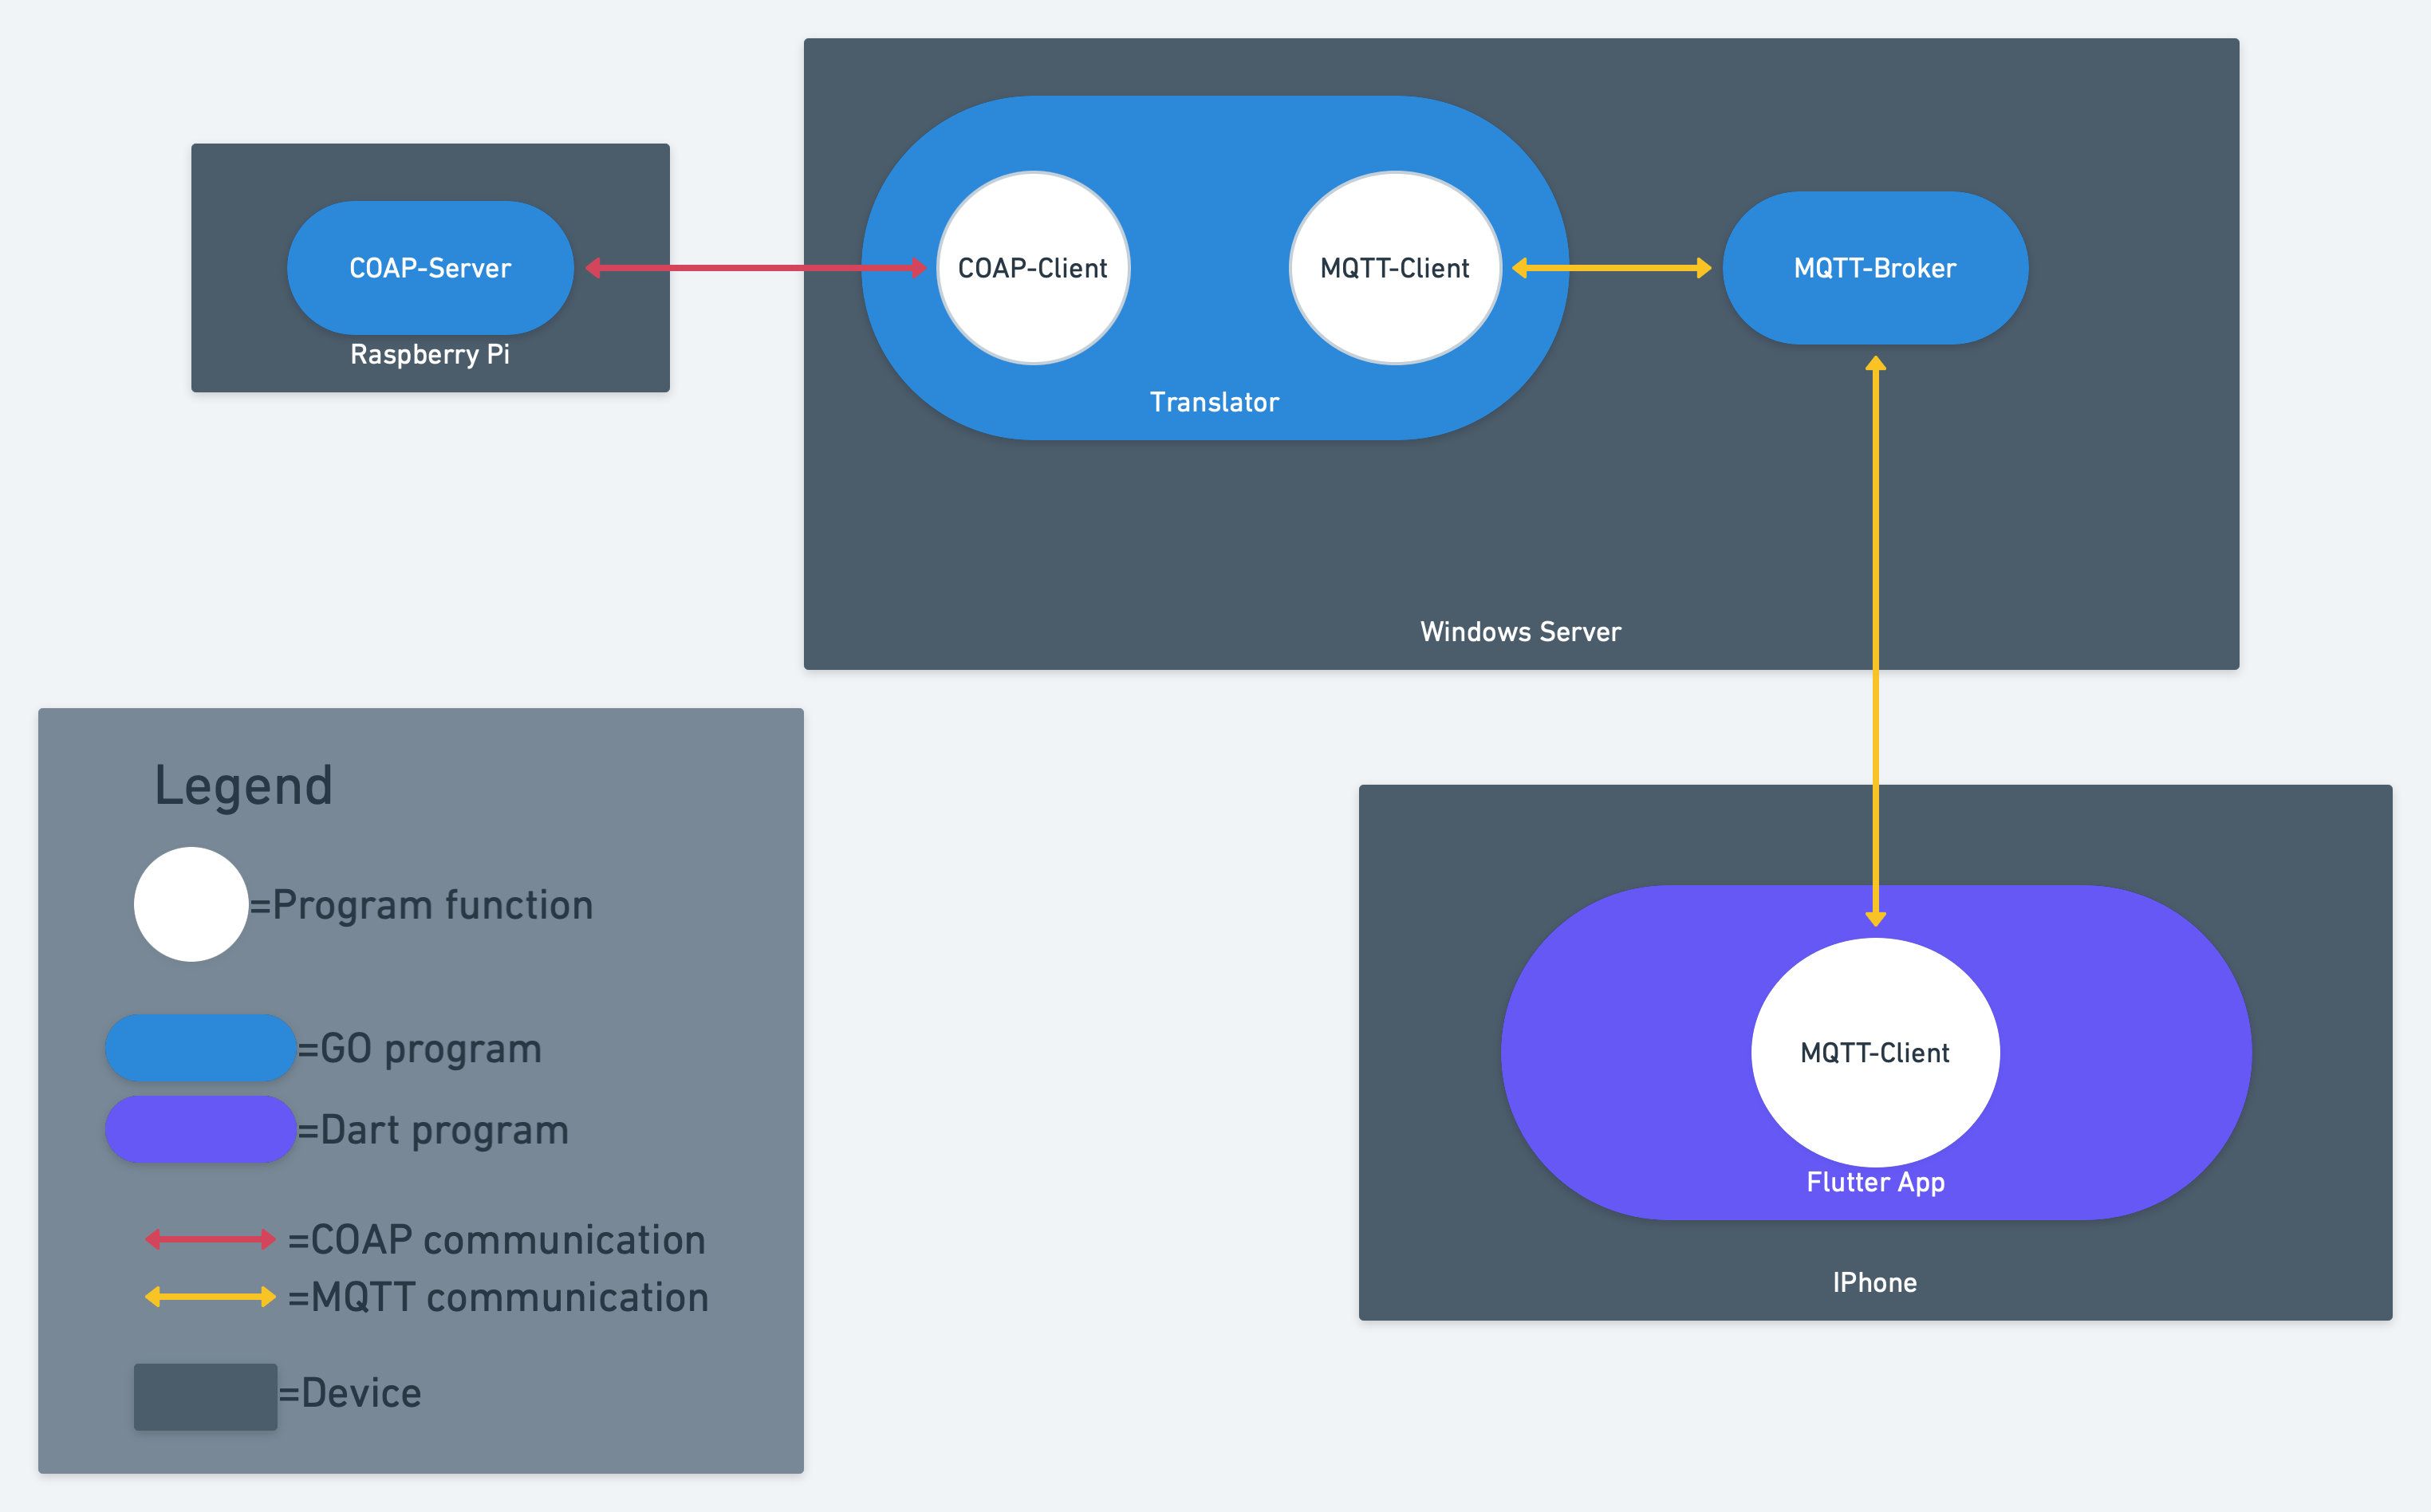
\includegraphics[width=1\textwidth]{img/communication.png} 
    \caption{The planned communication scheme. See legend for explanation}
    \label{fig:communication}
\end{figure}




With regards to C- and D-level diploma work, it is insufficient to merely perform a practical construction or programming project. A systematic study must also be carried out, e.g. an evaluation and analysis of the design or program. The study should result in objective facts, preferably in the form of tables and diagrams, into which your own conclusions are built in. The study can be a verification of a design that meets the requirement specification, or a comparison of competing alternatives. It is acceptable to allow users to answer a questionnaire or be interviewed. It is also possible to evaluate web-pages and other user interfaces according to usability criteria.

The method section is the point at which your chosen method and intended procedure during the research are discussed. This section shall not be a chronological diary filled with irrelevant details, but should contain information given in such a way that it is understandable for the reader and enables him/her to interpret your results and repeat your work, i.e. in order to check the results. Here, the tools, assumptions, mathematical models, performance measures and assessment criteria are presented. It is also at this point that the means adopted for the evaluation and verification of the computer programs and technical solution proposals are presented. This can include a test plan to check that the structure works and criteria to assess its usefulness. In research reports regarding natural science and technology this chapter is often called “Model”, “System Model” or “Simulation Model”.

Justify your choice of methodology/model. This choice is very important, because it could be the actual key to the result of your research. Comment on the method's possible weaknesses and problems that may arise during actual implementation. Refer to the problem wording in the introduction chapter. It is possible, for example, to write “problem P1 is attempted through the method M1 and problem P2 through…” 

In your report, you should - depending on what the report is about- find information about what you have investigated and how you have gathered and processed data. Possible questionnaires, interview questions and the likes can be presented as appendices. Detailed descriptions concerning experimental formats of possible interest to those wanting to repeat the experiment should also be included in this chapter.

    \section{Implementation}
\label{ch:impl}
\noindent	

\subsection{CoAP-server}
As mentioned in chapter \ref{ch:method:tech} the CoAP-server is implemented in Go using an external library \cite{goCOAP}. The library implements CoAP similarly to how Go normally handles HTTP. To start serving CoAP a router is created for routing request to different locations. A middleware was created to enable logging. The first rout added was the rout to get the mock temperature sensors. To create a rout an endpoint and a handler function needs to be provided to the router. In figure \ref{code:router} we can see the code snipped to create the router, add the middleware and lastly creating the first route.

\begin{figure}[H]
    \begin{lstlisting}[language=go]
r := mux.NewRouter()
r.Use(loggingMiddleware)
r.Handle("/temp", mux.HandlerFunc(handleTemp))
    \end{lstlisting}
    \caption{Go code snipped showing creating the CoAP router, adding a logging middleware and creating the handler for temperature}
    \label{code:router}
\end{figure}

The temperature handler decodes the incoming CoAP message to figure out what type of request it was. It also checks if the message has a payload. All the request types to this endpoint requires a payload. Figure \ref{code:temp:body} shows the code snippet for the initial handling of a request to the temperature endpoint. If the body does not exist it ends the request there by responding with bad request.
\begin{figure}[H]
    \begin{lstlisting}[language=go]
method := r.Code.String()
body := make([]byte, 128)
if r.Body == nil {
    w.SetResponse(codes.BadRequest, message.TextPlain, bytes.NewReader([]byte(string("No body included"))))
    return
}
n, _ := r.Body.Read(body)
body = body[:n]
\end{lstlisting}
    \caption{Code showing initial handling of the temperature request}
    \label{code:temp:body}
\end{figure}

The handler can handle 4 different request types: GET, POST, PUT, DELETE. 

GET responds with the current temperature of the processor if it exists otherwise it returns not found. Because the sensor is simulated, after the GET request it either increase or decrease the temperature of the sensor by a random amount between 1-3$^{\circ}C$. Figure \ref{code:temp:struct} shows the structure for a temperature sensor.

\begin{figure}[H]
    \begin{lstlisting}[language=go]
type TemperatureSensor struct {
    Status      bool
    Temperature int
    Location    string
}
\end{lstlisting}
    \caption{Structure for a mock temperature sensor}
    \label{code:temp:struct}
\end{figure}

POST creates a new temperature sensor. The request requires the payload to contain both the location of the sensor and the initial power status. When the request is received it creates a new instance of a temperature sensor. It assigns the values received and randomizes a temperature between -20-30$^{\circ}C$. If the request is successful it responded with status code created.

PUT request are used to switch power status. The request requires the body to contain the new power status and the name of the sensor to be changed. If the
sensor exists it changes its power status and responds with status Changed.

DELETE request removes a sensor if the payload includes the sensor name. If the request is successful it responds with Deleted.

For clients to be able to discover what temperature sensors is available the /all endpoint was created. This endpoint only accept GET request and uses Go's built in JSON library to convert the internal map of sensors to a JSON string to include in the response. The code implementation can be found in figure \ref{code:temp:all}.

\begin{figure}[H]
    \begin{lstlisting}[language=go]
r.Handle("/all", mux.HandlerFunc(func(w mux.ResponseWriter, r *mux.Message) {
    data, _ := json.Marshal(thermostats)
    w.SetResponse(codes.Content, message.TextPlain, bytes.NewReader(data))
}))
\end{lstlisting}
    \caption{Creation of the /all endpoint}
    \label{code:temp:all}
\end{figure}

The last endpoint is /pi which enables clients to gather information about the CoAP-server's processor and memory utilization. The server collects this data through the Linux proc files. CPU information is gathered through the proc/stat file while the memory is gathered through the proc/meminfo file. I used a library to help width parsing these files\cite{goProc}. A separate thread reads the proc files every second. For CPU usage it uses the last calculated value to derive the current usage in percentage. For the memory the proc/meminfo contains both free memory and total memory. From this the function derives the current usage in the format used/total.

\subsection{Translator}
The translator builds on a previous implemented CoAP client in Go. To translate from CoAP to MQTT a MQTT library was added to the project\cite{goMQTT}. The translator will poll data from the CoAP and then publish it to the MQTT-broker. It will also subscribe to certain MQTT messages to be able to convert them to CoAP request. The response from these messages will then be published.

The first thing the Translator does is send a request to the CoAP-server to retrieve the available sensor. This is to keep an internal map of what sensor are online to prevent the Translator to pull unnecessary data. After it retrieves the information about the temperature sensors it starts the connection to the MQTT broker and creates some constant subscriptions. When subscribing the MQTT library requires callback functions that will fire when a message is received to that topic. The connection code can be found in figure \ref{code:translator:connect}

\begin{figure}[H]
    \begin{lstlisting}[language=go]
populateSensors()
var broker = "localhost"
var port = 1883
opts := mqtt.NewClientOptions()
opts.AddBroker(fmt.Sprintf("tcp://%s:%d", broker, port))
opts.SetClientID("Coap Translator")

opts.SetDefaultPublishHandler(messagePubHandler)
opts.OnConnect = connectHandler
opts.OnConnectionLost = connectLostHandler
opts.SetPingTimeout(time.Second * 60)

client := mqtt.NewClient(opts)

if token := client.Connect(); token.Wait() && token.Error() != nil {
    panic(token.Error())
}
\end{lstlisting}
    \caption{Connection code for the Go MQTT client}
    \label{code:translator:connect}
\end{figure}

The constant subscription are: all, home/add, home/delete and home/change. The all topic is used for communication to the MQTT network the available temperature sensors. If an MQTT client publish a message with the structure GET:$id$. The Translator will get the information using the CoAP client and then forward the response to MQTT network via a publish message to the topic all/$id$. The function for parsing all the publish messages can be found in figure \ref{code:translator:all}

\begin{figure}[H]
    \begin{lstlisting}[language=go]
func allCallback(c mqtt.Client, m mqtt.Message) {
    message := string(m.Payload())
    fmt.Println(message)

    if strings.Contains(message, "GET") {
        split := strings.Split(message, ":")
        if len(split) != 2 {
            return
        }
        COAPmsg := createGet("all", "")
        payload := string(sendCreatedCoap(COAPmsg))
        fmt.Println(payload)
        tok := c.Publish("all/"+split[1], 0, false, payload)
        tok.Wait()
    }
}
\end{lstlisting}
    \caption{Function for parsing the /all endpoint}
    \label{code:translator:all}
\end{figure}

The home/add subscription is used to create a sensor. The Translator listens for publish messages and then relays the information to the CoAP-server. Figure \ref{code:translator:add} shows a code for the callback function to the home/add subscribe.

\begin{figure}[H]
    \begin{lstlisting}[language=go]
func addCallback(c mqtt.Client, m mqtt.Message) {
	message := string(m.Payload())
	msg := createPost("temp", message)
	payload := string(sendCreatedCoap(msg))
	fmt.Print(payload)
	populateSensors()
}
\end{lstlisting}
    \caption{Function for parsing the home/add publish}
    \label{code:translator:add}
\end{figure}

The home/change and home/delete functions similarly to home/add. home/change is used to change the power status of a temperature sensor and the home/delete is used to delete a temperature sensor. For all of these function the Translator repopulates the internal map to be up-to-date on what sensors exist and their power status

The main loop of the Translator is to first pull the temperature sensors if they are online. It then publishes this temperature to home/$id$. After it has taken care of the temperature it moves on to the CPU and memory information. It creates a request to the CoAP-server and then splits the information in to two publishes pi/cpu and pi/mem. When it has published the data it sleeps for 10 seconds and then starts from the top. The code for the main loop can be found in figure \ref{code:translator:loop}

\begin{figure}[H]
    \begin{lstlisting}[language=go]
for {
    for k, online := range sensors {
        if online {
            msg := createGet("temp", k)
            p := sendCreatedCoap(msg)
            tok = client.Publish("home/"+k, 0, true, p)
            tok.Wait()
        }
    }
    msg := createGet("pi", "")
    p := sendCreatedCoap(msg)
    //fmt.Println(string(p))
    tok = client.Publish("pi/cpu", 0, true, strings.Split(string(p), ":")[0])
    tok.Wait()
    tok = client.Publish("pi/mem", 0, true, strings.Split(string(p), ":")[1])
    tok.Wait()
    time.Sleep(time.Second * 10)
}
\end{lstlisting}
    \caption{The main loop of the Translator}
    \label{code:translator:loop}
\end{figure}

\subsection{Flutter mobile application}

    \section{Results}
\label{ch:results}
\noindent	
The results chapter is included when you have produced a systematic study, i.e. an evaluation of a program that you have developed, which is required for C - and D-level diploma work. In the results chapter objective results of the empirical study are presented. Keep in mind that possible comments in this chapter should only be used for clarification. Your own views and subjective (personal) comments belong in the chapter conclusion/discussion.

Strive to present the results, for example measurement-, calculations- and/or the simulation result, in a form that is as lucid and easily understandable as possible. The results are preferably presented in diagrams or tables. Accounts of interviews can be summarised, but may include concrete examples supporting your work.

Extensive results, for example complete summaries of survey results, large tables and long mathematical deductions, are placed in the appendices.

    \section{Discussion}
\label{ch:concl}
\noindent	
\subsection{Implementation}
\label{ch:concl:imp}
A complete system was implemented with working communication from a MQTT client in a user application to a CoAP-server running. There is one bug in the system that I have not found a solution for. Sometimes the Dart version of the MQTT-client sends a connect-message with identity 0 which is a reserved message ID. As I have not created it was hard to find the cause for this bug and I was not able to create a successful workaround. Luckily this does not happen often.

Another problem was that I was not able to fully utilize Flutters multi-platform support. The MQTT Dart library does support all platforms, but it requires different client objects for web applications. Dart does provide a check if the application is running on the web but including the package for the web version of the MQTT-client also adds a package that is not supported by the other platforms thus breaking the application for other platforms. 

By using Go for building everything is set up for concurrency, but I did not utilize it fully. Both the CoAP-server and the translator could be multithreaded using Go's concurrency features. This could theoretically decrease the latency.

\subsubsection{Other alternatives}
My implementation is not the only way to implement an end to end system for showing information from a remote device. Other alternatives could be using HTTP REST, WebSockets, pure CoAP and pure MQTT. 

Both MQTT and WebSockets offer an open bidirectional channel for communication between client and servers. The difference here is that MQTT has a structure for how clients send and receive messages. WebSockets on the other hand only is a standard for an open communication channel. When a client opens a WebSocket connection it can send and receive data. Underlying message structure is decided by the developer\cite{rfc6455}.

CoAP and HTTP REST work similarly. CoAP being designed to mimic the HTTP REST system. CoAP being more lightweight and is thus more suitable for IoT purposes. \cite{coapTech} Periodic data information this could be an alternative but for my application that have sensors that push data more frequently using one of these technologies would mean sending more requests periodical instead of getting the information when it is published.

If I were to build this again I would aim for a purely MQTT system and remove CoAP. If I was dealing with more sparse update on the IoT data, then CoAP would be better suited due to the system not updating as often.


\subsection{Results}
In the figure \ref{fig:bench2} and figure \ref{fig:bench3}. We can see that when the application is compiled for macOS it has overall the worst latency in terms of mean, max and standard deviation. It is expected for the result to be different depending on what applications request reach the broker first. But I also think that due to Flutter not being able to compile to ARM binaries for macOS and thus the macOS version of the application running on a compatibility layer could affect the results.

Looking at all the benchmark runs side by side the mean and max values does not change drastically except for the macOS case. Comparing figure \ref{fig:bench1:dev1}, figure \ref{fig:bench2:dev1} and figure \ref{fig:bench3:dev1} we can see that from benchmark run 1 to run 2 the number of request per second decrease from about 28 to about 23. But from run 2 to run 3 we only see a change from about 23 to 22. Similar changes can be seen in the other metrics as well, a bigger change between run 1 and run 2 but a smaller change between run 3 and 4. 

To get a better understanding on how the system scales I would like to write a Go program that can generate x amount of Clients in separate threads to emulate more clients sending and receiving data. Due to the time limitation of this project I was not able to create this. Lastly as I mentioned in chapter \ref{ch:concl:imp} multi threading is possible on both the Translator and CoAP-server. It would be interesting to see how this changes the RTT.

\subsection{Ethical and Societal Discussion}
\label{ch:concl:ethical}
When talking about IoT as a whole I think it is important to talk about privacy concerns. A lot of IoT systems for consumers are built on cloud technologies for a fluid user experience, and one thing I keep in mind is if the cloud service the company uses for their IoT devices is free then the user data is the product. 

With this project I am now able to implement IoT Protocols and if I want to avoid my data being collected I could just implement my own smart home. The problem here is we cannot expect the average consumer to do this. Thus, the consumer must be aware of what product collects data and how it is handled by the producer.

\subsection{Future Work}
\label{ch:concl:future-work}
First improvement I would make is to enable multithreading on both the Translator and the CoAP-server. This would theoretically improve the RTT due to both the Windows Server running the Translator and the Raspberry Pi running the CoAP-server having multiple cores to process requests on. 

To better evaluate the system I would like to implement a program in Go that uses multiple threads to simulate more clients. With the multiple clients in the same program it would be easier to calculate metrics based on all clients RTT instead of each client on its own.

In the end I would ideily remove CoAP from the system completely because I do not think it contributes much to the system. For now the system runs on "stable" hardware with every component except the Flutter application running on hardwired Ethernet.

    \printbibliography
    \newpage
    \pagestyle{empty}
    
    \pagestyle{fancy}
    \appendix
    \noappendicestocpagenum
    \setcounter{page}{1}

    \counterwithin{figure}{section}
    \counterwithin{table}{section}


    \begin{appendices}
      \section{Source Code}
\label{appendix:source-code}
    \end{appendices}

\end{document}
